\chapter{Classical construction/update/destruction algorithm \Author{J. Singer \andAuthor F. Rastello}}
\label{chap:classical_construction}
\inputprogress

\graphicspath{{Figures/}{classical_construction_algorithm/Figures/}{part1/classical_construction_algorithm/Figures/}}


\def\phiops{$\phi$-functions}
\def\phiop{$\phi$-function}

%% jsinger additions
\def\undef{\perp}
\def\DF{\mathrm{DF}}
\def\iDF{\mathrm{iDF}}
\def\join{\cup}

%% jsinger - simple introductory paragraphs

This chapter describes the standard algorithms for construction and
destruction of SSA form.

SSA \emph{construction} refers to the process of translating a non-SSA program into
one that satisfies the SSA constraints. In general, this transformation
occurs as one of the
earliest phases in the middle-end of an optimizing compiler, when the program
has been converted to three-address intermediate code.
SSA \emph{destruction} is sometimes called out-of-SSA translation. This phase
generally
takes place in an optimizing compiler after all SSA optimizations have
been performed, and prior to code generation. However note that there are
specialized code generation techniques that work directly on SSA-based
intermediate representations such as code selection (see Chapter~\ref{chapter:code_selection}), if-conversion (see Chapter~\ref{chap:if_conversion}), or register allocation (see Chapter~\ref{chap:register_allocation}).

The algorithms presented in this chapter are
based on material from the seminal research papers on SSA.
These original algorithms are 
straightforward to implement and have acceptable efficiency.
For these reasons, the algorithms
are widely implemented in current compilers.
Note that more
efficient, albeit more complex, alternative algorithms have been devised.
These are described further in Chapters 
\ref{chap:alternative_ssa_construction_algorithms}
and
\ref{chap:alternative_ssa_destruction_algorithm}.

Throughout this chapter,
we assume that a `program' is represented as an
intra-procedural control flow graph (CFG)
with a single entry node $r$, from which every other
node is reachable.
Data flow occurs through definitions and uses of 
variables, with no pointer indirection.
%% FIXME - forward reference to Part II ...
(Part II of this textbook contains chapters dealing with
SSA extensions for high-level features like
pointer-based aliasing, arrays, compound data structures, concurrency, etc.)

Figure \ref{fig:examplecfg} shows an example CFG 
program. The set of nodes is $\{ r, A, B, C, D, E\}$.
The set of variables is $\{ x, y, \mathit{tmp} \}$.
Note that the program shows the complete control flow structure,
denoted with directed edges between the nodes.
However the program only shows 
statements that define relevant variables, together with the
unique \texttt{return} statement at the exit point of the CFG.
All of the program variables are undefined on entry. On certain
control
flow paths, some variables may be used without being defined.
We discuss this issue later in the section.
We intend to use this program as a running example
throughout the chapter,
to demonstrate various aspects of SSA construction.


\begin{figure}
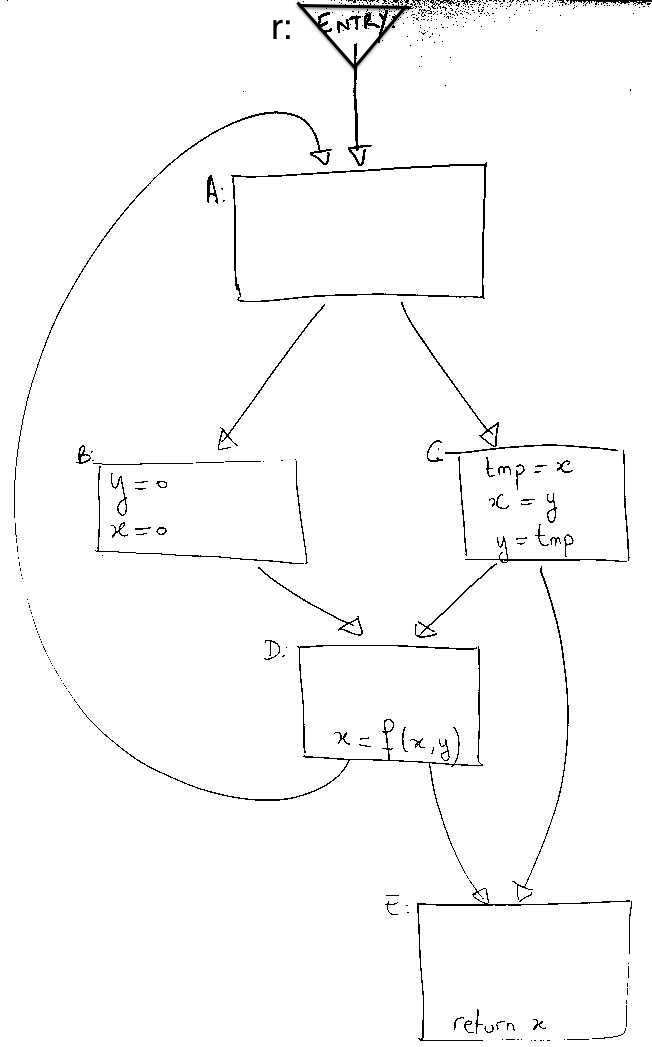
\includegraphics[width=5cm]{initial.jpg}
\caption{\label{fig:examplecfg}Example control flow graph, before
  SSA construction occurs}
\end{figure}

\section{Construction}
The original construction algorithm for SSA form 
consists of two distinct phases.
\begin{enumerate}
\item \textbf{\phiop\ insertion} performs \textit{live-range splitting} to ensures that any use of a given variable $v$ is reached~\footnote{A program point $p$ is said to be \emph{reachable} by a definition of $v$, if there exists a path in the CFG from that definition to $p$ that does not contain any other definition of $v$.}  by exactly one definition of $v$. 
The resulting live-ranges exhibit the property of having a single definition, which occurs at the beginning of each live-range.
\item \textbf{variable renaming} assigns a unique variable name to each live-range. This second phase rewrites variable names in program statements such that the program text contains only one definition of each variable, and every use refers to its corresponding unique reaching definition.
\end{enumerate}

As already outlined in Chapter \ref{chap:properties_and_flavours},
there are different flavors of SSA with distinct properties.
In this chapter, we focus on the \textit{minimal} SSA form.
Construction of minimal SSA 
requires for each variable $v$ the insertion of \phiops\ at $\join(D_v)$.
Here $D_v$ is the set of definition points of $v$, and,
for a given set of program points $S$, $\join(S)$ is the set of
\textit{join nodes} of $S$
i.e., nodes in the CFG that can be reached by
two (or more) distinct elements of $S$ using disjoint paths.

Let us consider some join set examples from the
program in Figure \ref{fig:examplecfg}.
\begin{enumerate}
\item $\join(\{B,C\}) = \{D\}$, since it is possible to get from $B$ to $D$
and from $C$ to $D$ along different, non-overlapping, paths.
\item Again, $\join(\{r, A, B, C, D, E \}) = \{A,D,E\}$, since the nodes
$A$, $D$, and $E$ are the only nodes with multiple predecessors in
the program.
\end{enumerate}

 
The original construction for SSA form uses an over-approximation of
join sets, the iterated dominance frontier $\iDF(S)=\join(S\cup
\{r\})$, i.e.\ it assumes an \emph{implicit} definition of every
variable at the entry node $r$.
The iterated dominance frontier is the limit of the sequence:
$$\begin{array}{lll}
\DF_1(S) & = & \DF(S)\\
\DF_{i+1}(S) & = & \DF\left(S\cup \DF_i(S)\right)
\end{array}$$

% described dominance frontiers? In chapter 2?
Recall the definition of dominance frontiers from Section
\ref{sec:properties:domfrontiers}.
Informally, the dominance frontier of a node $n$, $\DF(n)$,
is the border of the CFG region that is dominated by $n$.
Also note that $\DF$ is defined over individual nodes, 
but for simplicity of presentation, we overload it to 
operate over sets of nodes too, i.e.\ 
$\DF(\{n_a,n_b\}) = \DF(n_a) \cup \DF(n_b)$.

We end up with a straightforward algorithm that places \phiops\
on a per-variable basis.
For a given variable $v$, we place \phiops\ at the
iterated dominance frontier $\iDF(S)$ where
$S$ is the set of definition points for $v$.
As discussed earlier, this leads to building a form that has
the dominance property (see Chapter~\ref{chapter:properties_and_flavors}).

Consider again our running example from Figure 
\ref{fig:examplecfg}. The set of definition points for variable
$x$ is $\{ B,C,D \}$. The iterated dominance frontier of this set
is $\{ A, D, E \}$. Hence we need to insert 
\phiops\ for $x$ at the heads of nodes $A$, $D$, and $E$.
Figure \ref{fig:examplecfg_varx} shows the example CFG program
with inserted \phiops\ for $x$ marked in red.

\begin{figure}
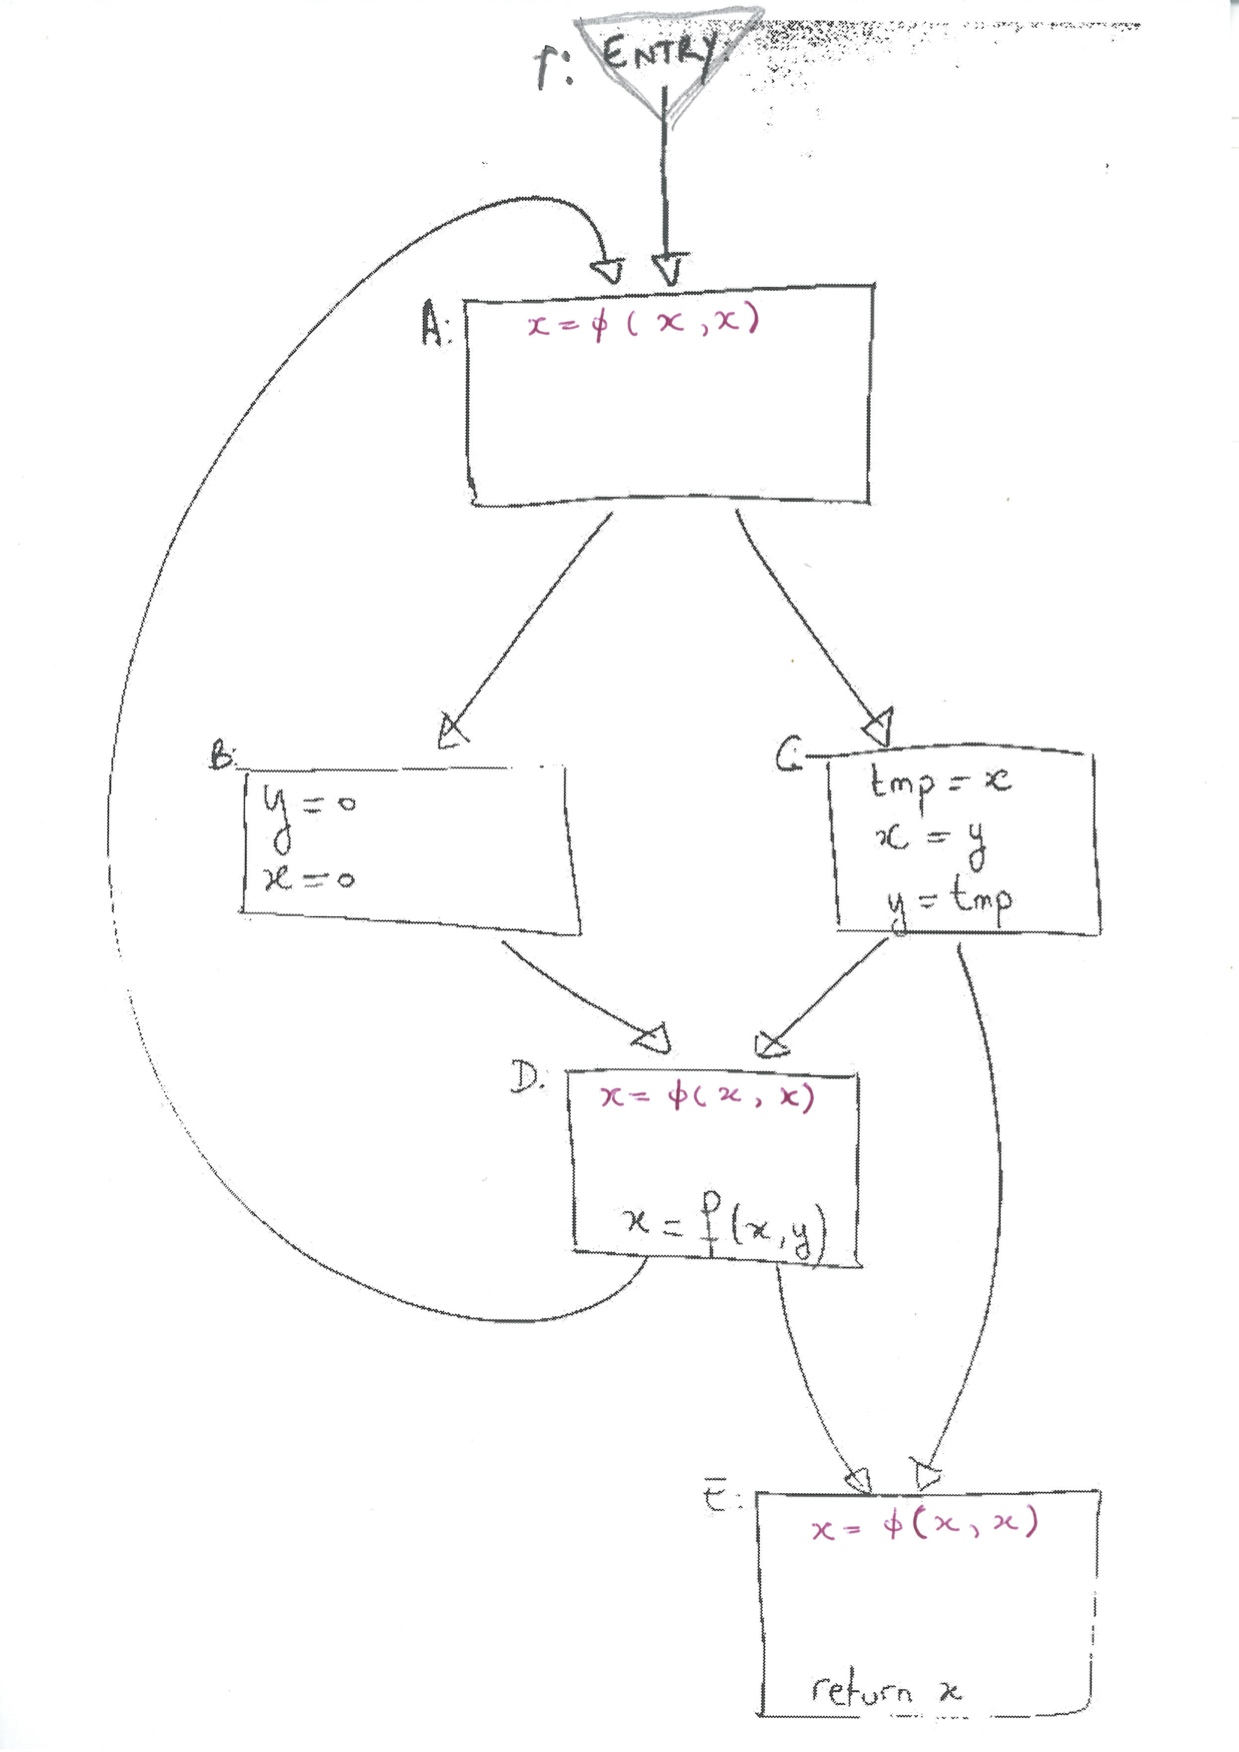
\includegraphics[width=5cm]{ssa_variablex.jpg}
\caption{\label{fig:examplecfg_varx}Example control flow graph, including
inserted \phiops\ for variable $x$
}
\end{figure}



As far as the actual algorithm for \phiops\ insertion
is concerned, we assume that the dominance
frontier of each CFG node is precomputed. However
it is not reasonable to assume that the iterated dominance frontier is
precomputed.
Thus the iterated dominance frontier is computed just-in-time,
as the algorithm proceeds.
The algorithm works by inserting \phiops\ iteratively
using a worklist of definition points, and flags (to avoid multiple
insertions). The corresponding pseudo-code is given in
Algorithm~\ref{alg:classical_construction:phi_insertion}.

Since a \phiop\ is itself a 
definition, it may require further \phiops\ to be inserted.
This is the cause of node insertions into the  worklist $W$ during
the iterations of the inner loop.
Effectively, this is the just-in-time construction of
the iterated dominance frontier.

The worklist of nodes $W$ is used to record definition points that the
algorithm
has not yet processed, i.e.\ it has not yet inserted \phiops\ at their dominance
frontier.
The flags array $I$ is used to avoid repeated insertion of \phiops. Dominance
frontiers
of multiple nodes may intersect, e.g.\ $\DF(B)$ and $\DF(C)$ both contain $D$. 
Once a \phiop\ for a variable has been
inserted, there is no need to insert another, since a single \phiop\ per
variable handles all incoming definitions of that variable.

Table \ref{tab:classical_construction:walkthru} 
gives a walkthrough example of the Algorithm 
\ref{alg:classical_construction:phi_insertion} for inserting \phiops\ for $x$.
At the beginning, the CFG looks like Figure \ref{fig:examplecfg}.
At the end, when all the \phiops\ for $x$ have
been placed, then the CFG looks like Figure \ref{fig:examplecfg_varx}.
\emph{FIXME - should we include a graphic showing
the CFG state at intermediate phases 
in the walkthrough?}

\begin{table}
\begin{center}
\begin{tabular}{r|c|c|p{5cm}}
\textbf{iteration} & $W$ & $I$ & \textbf{actions} \\ \hline 
init & $\{\}$ & $\{\}$ & insert $B$, $C$ and $D$ into both $W$ and $I$, since
$B$, $C$ and $D$ are
definition points of variable $x$ \\
0 & $\{B,C,D\}$ & $\{B,C,D\}$ & remove $B$ from $W$ for processing, 
$\DF(B)$ contains only $D$, so insert \phiop\ for $x$ at $D$. Since $D$ is
already in $I$ we do not need to reinsert it into $W$ or $I$. \\
1 & $\{C,D\}$ & $\{B,C,D\}$ & remove $C$ from $W$ for processing,
$\DF(B)$ contains both $D$ and $E$, $D$ already has a \phiop\ for $x$, so do
nothing more for $D$. $E$ does not have a \phiop\ for $x$, so insert
one. Add $E$ to both $W$ and $I$. \\
2 & $\{D, E\}$ & $\{B,C,D,E\}$ & remove $D$ from $W$ for processing,
$\DF(D)$ contains both $A$ and $E$. $A$ does not have a \phiop\ for
$x$, so insert one. Add $A$ to both $W$ and $I$. Since $E$ already
has a  \phiop\ for $x$, do nothing more. \\
3 & $\{E,A\}$ & $\{B,C,D,E,A\}$ & remove $E$ from $W$ for processing, 
$\DF(E)$ is empty since $E$ is the exit node of the CFG, so do
nothing. \\
4 & $\{A\}$ & $\{B,C,D,E,A\}$ & remove $A$ from $W$ for processing, 
$\DF(A)$ is empty since $A$ dominates all nodes in the CFG, so do
nothing. \\
5 & $\{\}$ & $\{B,C,D,E,A\}$ & $W$ is empty so the algorithm
moves onto the next variable. \\
\end{tabular}
\end{center}
\caption{\label{tab:classical_construction:walkthru}Walkthrough of
  placement of \phiops\ for variable $x$ in example CFG}
\end{table}

% To illustrate this point, in the running example CFG, Figure
% Figure \ref{fig:examplecfg_varx},
% the \phiop\ for $x$ at node $E$ could have been inserted because $E$
% is in the dominance frontier of $D$. However $E$ is also in the dominance
% frontier of $C$. Once
% the \phiop\ for $x$ has been inserted at $E$, there is no need
% to reinsert it or 
% to reprocess nodes in $\iDF(E)$.


(FIXME - do we need the next paragraph here or should we leave this detail until
the Advanced construction chapter??)

Providing the dominance tree as a given, the computation of the dominance frontier is quite straight-forward. This can be understood using the DJ-graph notation. The skeleton of the DJ-graph is the dominator tree of the CFG that makes the $D$-edges. This is augmented with $J$-edges (join edges) that correspond to all edges of the CFG which source do not dominate its destination. A $DF$-edge (dominance frontier edge) is an edge which destination is in the dominance frontier of its source. By definition, there is a $DF$-edge $(a,b)$ between every CFG nodes $a$, $b$ such that there is a CFG-path from $a$ to $b$ but $a$ does not dominate $b$. 
In other-words, for each  $J$-edge $(a,b)$, all ancestors (including $a$) that do not dominate $b$ have $b$ in their dominance frontier. This leads to the pseudo-code given in Algorithm~\ref{alg:classical_construction:df}. The iterated dominance frontier is nothing else than the transitive closure of the dominance frontier and we can define the $DF^+-graph$ as the transitive closure of the $DF$-graph. We can compute the iterated dominance frontier for each variable independently, as proposed in this chapter, or ``cache'' it to avoid multiple computation of the iterated dominance frontier of the same node. This leads to more sophisticated algorithms detailed in Chapter~\ref{chap:alternative_ssa_construction_algorithms}.

\begin{algorithm}
\Begin{
 \For{$(a,b) \in cfgEdges$}{
  \While{not a dominate b}{
     $\DF(a) \leftarrow \DF(a) \cup b$\;
     $a \leftarrow \mathrm{iDom}(a)$\;
  }
 }
}
\caption{\label{alg:classical_construction:df}Algorithm for computing the dominance frontier of each CFG node}
\end{algorithm}

\begin{algorithm}
\Begin{
 $W \leftarrow \{ \}$ : set of basic blocks\;
 $I \leftarrow \{ \}$ : set of basic blocks\;
 \For{$v$ : variable names in original program}{
  \For{$d$ : definition statements of variable $v$}{
    \textbf{let} $B$ be the basic block containing $d$\;
     $W \leftarrow W \cup \{ B \}$\;
     $I \leftarrow I \cup \{ B \}$\;
  }
  \While{$W \neq \{\}$}{
   remove a basic block $X$ from $W$\;
   \For{$Y : \mbox{basic block} \in \mathrm{DomFrontier}(X)$}{
    \If{$Y$ does not contain a $\phi$-function for $v$}{
        add $v \leftarrow \phi(...)$ at start of $Y$\;
        \If{$Y \notin I$}{
          $W \leftarrow W \cup \{ Y \}$\;
          $I \leftarrow I \cup \{ Y \}$\;
        }
     }
    }
  }
}
}
\caption{\label{alg:classical_construction:phi_insertion}Standard algorithm for inserting $\phi$-functions}
\end{algorithm}


Once \phiops\ have been inserted using this algorithm, the program may
still contain several definitions per variable, however now there is a
single definition statement 
in the CFG that reaches each use. Moreover, with the following semantics for \phiops\ where its variable uses are considered to be on the corresponding predecessor basic blocks, then use-def chains are aligned with the CFG dominance tree. In other word the unique definition that reaches each use dominates that use.

To obtain the desired property of a static single assignment per variable,
it is necessary to perform variable renaming.
Because of the dominance property outlined above,
renaming can be easily achieved using a depth-first traversal of the dominance tree.
During the traversal, for each variable $v$, it is necessary to remember its nearest dominating definition.
This gives the following pseudo-code for the variable renaming algorithm:

\begin{verbatim}
proc renaming:
// rename variable def and use to have one definition per variable
  foreach v: Variable
    let v.reachingDef:=undef
  foreach B: basicBlock in DFS preorder of the dominance tree
    foreach inst: instruction from top to bottom of B
      foreach o: a use operand of inst
        let v the variable used in o
        v.update_reachingDef(o)
        replace v by v.reachingDef in o
      foreach o: a def operand of inst
        let v the variable used in o
        v.update_reachingDef(o)
        create new variable v'
        replace v by v' in o
        v'.reachingDef:=v.reachingDef
    foreach phi: phi instruction in a successor of B
      foreach o: a use operand of phi
        let v the variable used in o
        v.update_reachingDef(o)
        replace v by v.reachingDef in o
\end{verbatim}

\begin{verbatim}
proc v.update_reachingDef(o):
// simply go up along the reachingDef chain until dominance is fulfilled 
  let rd:=v.reachingDef
  while not (rd==undef || def(rd) dominates o)
    rd:=rd.reachingDef
  v.reachingDef:=rd
\end{verbatim}

Let us review the flavour of SSA form that can is constructed by this simple
algorithm. (FIXME - Ref back to chapter 2?)
\begin{itemize}
\item It is \textit{minimal} --- FIXME what does minimal mean? 
\item It is \textit{not pruned} SSA as some dead \phiops\ are possibly inserted.
\item It is \textit{conventional} SSA as the transformation that renames back all $\phi$-related variables into a unique representative one, and removes all \phiops\ is a correct SSA-destruction algorithm.
\item Finally, it has the \textit{dominance} property; each variable use is dominated by its unique definition. This is due to the use during the $\phi$-placement phase of iterated dominance frontier instead of join set. Whenever the iterated dominance frontier of the set of definition points of a variable differs from the join set, then at least one program point can be reached both by $r$ (the entry of the CFG) and one of the definition points. In other words, as in the double diamond figure (to be inserted), a use of an inserted \phiop\ does not have any actual reaching definition that dominates it. This corresponds to the undef value used to initialize reachingDef in the renaming phase pseudo code. Actual implementation can use NULL value, create a fake undefined variable at the entry of the CFG, or create on the fly undef pseudo operations just before the concerned used. We choose to use in this book the undef value, represented with the $\undef$ sign.
\end{itemize}


\section{Destruction \Author{F. Rastello}}
\label{sec:classical_destruction}

SSA form is a simple and efficient means of
sparsely representing program information used for code analysis and optimization. Once we have completed SSA based optimizations, or at least before code generation, we need to get rid of \phiops\ that are not machine instructions. This phase is called SSA destruction. 
Destructing freshly constructed SSA code is easy. One simply has to first rename back into a unique representative variable all $\phi$-related variables (which we refer to as \textit{SSA-webs}) that had initially the same name. Then each \phiop\ that has all its operands identical can be removed to coalesce the related live-ranges.
Finding SSA-webs can be performed efficiently using the classical union-find algorithm for merging sets:
\begin{verbatim}
proc find_webs
// find the ssa web of each variable
foreach variable v:
  ssaweb(v) := {v}
foreach instruction of the form "a=phi(a1,...,an)"
  foreach ai union(ssaweb(a),ssaweb(ai))
\end{verbatim}

An SSA form is said to be conventional if for each SSA-web, all its variables can be safely renamed into a unique representative one. In other words each SSA-web should be interference free. While freshly constructed SSA code is conventional, this may not be the case after optimizations such as copy folding FIXME - copy propagation???  have been performed.

The simplest (but not the most efficient) way for destructing non conventional SSA form is to split all (critical) edge, and then replace \phiops\ by parallel copies on predecessor blocks. By splitting an edge say ($s,d)$, we mean replacing it by an edge from $s$ to a freshly created basic block and by another edge from this new basic block to $d$. The corresponding pseudo-code is the following:

\begin{verbatim}
foreach B0: basic block of the CFG
  let PC0:= "{}" be an empty parallel copy instruction
  insert PC0 at the beginning of B0 just after the phi instructions
  let (B1,...,Bn) be the list of basic blocks predecessors of B0
  foreach Bi
    let PCi:= "{}" be an empty parallel copy instruction
    if Bi has several successors
      create basic block B'i
      replace edge Bi->B0 by Bi->B'i & B'i->B0
      insert PCi in B'i
    else
      append PCi at the end of Bi
    
  foreach phi instruction at the entry of B of the for "a0=phi(B1:a1,..,Bn:an)"
    let a' be a freshly created variable
    add copy "a0<-a'" to PC0
    replace a0 by a' in the phi instruction
    foreach ai (argument of the phi corresponding to Bi)
      add copy "a'<-ai" to PCi
      replace ai by a' in the phi instruction
    remove the phi instruction (otherwise get conventional SSA)
\end{verbatim}


Even this extremely conservative algorithm can lead to potential bugs especially when dealing with SSA destruction at code generation level. Indeed, we must make sure that appending a copy at the very end of a basic block is possible. This would, for example be problematic, in the situation where the jump at the end of the basic block defines a variable used in the following \phiop. We should also be careful of duplicated edges, ie when a basic block appears twice in the list of predecessors. This can append after some dead code and empty block eliminations. In that case, the edges should be considered as critical and then split.

We should outline that this technique has several drawbacks: first because of specific architectural constraints, region boundaries, or exception handling code, the compiler might not allow to split a given edge; second, the obtained code contains many additional temporary-to-temporary copies. In theory, coping with these copies is the role of the coalescer during the register allocation phase. But only decoupled register allocators (such as the one detailed in Chapter~\ref{chap:register-allocation}) with memory and time-consuming coalescing heuristics can handle the removal of these copies effectively. Coalescing can also, with less efforts, be handled prior to the register allocation phase. As opposed to a (so called conservative) coalescer during register allocation, this so called aggressive coalescing would not cope with the interference graph colorability. Still the insertion of copies itself might take a substantial amount of time and might not be suitable for dynamic compilation. The goal of Chapter~\ref{chap:alternative-destruction} is to cope both with non splittable edges and difficulties related with SSA destruction at machine code level, but also aggressive coalescing in the context of resource constrained compilation.

Once, \phiops\ have been replaced by parallel copies, we need to sequentialize parallel copies ie replace them by a sequence of simple copies. This phase can be performed right after SSA destruction or later on even after register allocation have been performed (see Chapter~\ref{chap:register_allocation}). It might be useful to postpone it as it introduces some arbitrary interferences between variables. As an example, $(a_1,b_1)\gets (a_2,b_2)$ can be sequentialized into $a_1\gets a_2;\ b_1\gets b_2$ which would make $b_2$ interfere with $a_1$ while the other way round $b_1\gets b_2;\ a_1\gets a_2$ would not ($a_2$ would interfere with $b_1$ instead).
If we still decide to replace parallel copies into a sequence of simple copies right after our SSA destruction (with no copy propagation / coalescing in between), this is straightforward: as no variable both appears as a source and as a destination (either all the sources or all the destinations are freshly created variables), any order is correct. Chapter~\ref{chapter:alternative_ssa_destruction_algorithm} will provide the pseudo-code that is required after coalescing have been performed and Chapter~\ref{chapter:register_allocation} will deal with the case under register allocated code.

\section{Turning general SSA into minimal/conventional/pruned/dominance property}

As discussed in Chapter~\ref{chapter:properties_and_flavours}, SSA can come in different flavors. It may or may not be conventional (each SSA web is interference free); it may or may not fulfill the dominance property (each variable definition dominates all its uses); it may or may not be pruned (does not contain any dead \phiop); it may or may not be minimal (there is no ``identity'' \phiops).
This section is devoted to the description of algorithms that turn SSA into the desired flavor.

Making SSA conventional, precisely corresponds to the first phase of SSA destruction (described in Section~\ref{sec:classical_destruction}) that splits critical edges and introduces parallel copies (sequentialized later on or on the fly) around \phiops. As already discussed, this straightforward algorithm has several drawbacks addressed in Chapter~\ref{chapter:chapter:alternative_ssa_destruction_algorithm}.

Making SSA strict ie fulfill the dominance property, is as ``hard'' as constructing SSA. Of course, a pre-pass can detect the variables which definitions do not dominate their uses, but basically one of the numerous possible variable per variable \phiops\ insertion algorithm (see Chapter~\ref{chapter:alternative_ssa_construction_algorithms}) can be used by restricting them to the set of interesting variables. The renaming phase can also be used with the same filtering process. As the number of variables to repair, might be a small proportion of all variables, a costly traversal of the whole program can be avoided by building the def-use chains (the non dominating ones) during the detection phase. Renaming can then be done in a variable per variable basis or better (if pruned SSA is preferred) the reconstruction algorithm presented in Chapter~\ref{chapter:repair_maintain_ssa_after_optimization} can be used both for renaming and \phiops\ placement.

The construction algorithm described in this chapter does not build pruned SSA form. It can easily be modified to build a so called semi-pruned SSA form by simply filtering out the local variables ie variables which definitions dominate there uses and appear in the same basic block. Then, if liveness information is available prior to the construction, it can be used to filter out the insertion of \phiops\ wherever the variable is not live.
If the original liveness information is not available, pruning SSA form is nothing else than dead-code elimination. As use-def chains are explicitly provided by SSA form is simply relies in marking actual uses (non \phiops\ ones) as useful and propagate backward through \phiops usefulness. This leads to the following pseudo-code:

\begin{verbatim}
stack = ()
foreach I: instruction of the CFG in dominance order
  if I of the form "a=phi(...)"
    mark a has useless
  else I of the form "...=f(a1,...,an)"
    foreach ai defined by a phi function
      mark ai as useful
      stack.push(ai)
while a := stack.pop
  let I: "a=phi(a1,...,an)" be the phi-function that defines a
  foreach ai marked as useless
    mark ai as useful
    stack.push(ai)
foreach I: phi instruction of the form a=phi(...)
  if a marked as useless then delete I  
\end{verbatim}

Construction of Minimal SSA comes with the price of a sophisticated algorithm involving iterated dominance frontier. 
Still, \phiops\ placement could be done pessimistically, as described further, on each CFG nodes along the live-ranges of the variables (or at every basic-block if we are extremely lazy or simply do not want SSA to be pruned). 
Also, code transformations such as code motion, CFG modifications, can make a minimal SSA non minimal.
Actually, minimality can be obtained/recovered using copy propagation whenever the CFG is reducible. 
To be efficient (as otherwise as many iterations as the maximum loop depth might be necessary), def-use chains should be computed. 
As already mentioned in Chapter~\ref{chapter:properties_and_flavours}, copy propagation can break the dominance property by propagating variable $a$ through \phiops\ of the form $a'=\phi(a_1,...,a_n)$ where $a_i$ are either equal to $a$ or $\undef$. 
If we want to avoid breaking the dominance property we simply have to avoid the use of this simplification rule that involves $\undef$. 
A more interesting rule is the one that propagates $a$ through a \phiop\ of the form $a'=\phi(a_1,...,a_n)$ where $a_i$ is either equal to $a$ or $a'$. 
``Identity'' \phiops\ can be simplified this way from inner to outer loops. 
Actually, when the CFG is reducible, this leads to minimal SSA. 
The underlying reason for that is that the def-use chain of a given variable is in this context a sub graph of a reducible graph: 
all nodes but those that can be reached by two different paths (from actual non \phiops\ definitions) can be simplified using iteratively $T1$ (merge of a node to its unique predecessor) or $T2$ (removal of self edge) reductions.
More precisely:
\begin{itemize}
\item simplifying any \phiop\ $a'=\phi(a_1,...,a_n)$ such that all $a_i$ are equals corresponds to $T1$ reduction
\item simplifying any \phiop\ $a'=\phi(a_1,...,a_n)$ such that each $a_i$ is either equal to $a'$ or to $a_1$, corresponds to $T2$ followed by $T1$ reduction.
\end{itemize}
This leads to a worklist algorithm in which the worklist stores the nodes that might be simplified. The worklist can be initialized with successors of non-\phiops\ definitions of variables (sources of the graph) -- if we want to stick on the framework of graph reduction --, or simply with all \phiops. Of course, if loop nesting forest is available, worklist can be avoided by traversing the CFG in a single pass from inner to outer loops, and in a topological order within each loop (header excluded)... 
As we believe the main motivation for this approach to be its simplicity, the pseudo-code provided here uses a worklist:

\begin{verbatim}
worklist := ()
foreach I: phi instruction of the program
  worklist.push(I)
  mark I
while worklist is non empty
  unmark I
  I := worklist.shift
  let I be of the form a'=phi(a1,...,an)
  if foreach ai, ai in {a1,a'}
    foreach I': instruction different than I that uses a'
      replaces a' by a1 in I'
      if I' not marked
        mark I'
        worklist.push(I')
\end{verbatim}


\section{Additional reading}

The early literature on SSA form
\cite{cytron89efficiently,cytron91efficiently}
introduces the construction algorithm we have outlined in this chapter,
and discusses its algorithmic complexity on common and worst-case inputs.

There are numerous published descriptions of alternative algorithms.
One of the most unconventional, which is striking for its elegant simplicity,
is presented by Aycock
and Horspool \cite{aycock00simple}. 
This is a pessimistic SSA construction technique,
in that it initially assumes $\phi$-functions are required
for all variables at all control flow merge points. 
It proceeds to remove unnecessary $\phi$-functions 
using simple rewrite rules.

Sreedhar and Gao \cite{sreedhar95linear} pioneered
linear-time complexity construction algorithms based on DJ-graphs.
Their work has since been refined by other researchers.
Chapter \ref{chap:alternative_ssa_construction_algorithms}
explores these more efficient algorithms in depth.


%%% FAB: we should probably move the technical discussions to this part?
%%% At least, put all the external references here (eg Cytron, etc.)
%%% TODO: write this section
Should cite (at least):
\begin{itemize}
\item Cytron for original construction and Aycock for minimality/simple construction and also reference to Semantic chapter (for minimality they have a similar copy-prop algo in the context of functional programming; for construction and dominance notion they have a nice equivalence with functional programming again) 
\item Wolf (J+=J) for join set
\item Sreedhar Gao (linear time algo) for properties on DJ-graphs, DF-graphs and dominance tree \& Ramalingam (loops, dom, dom-tree) for loop nesting forest dom-tree and DF \& reference to advanced SSA construction
\item Sreedhar's paper \& Glessner for basic correct SSA destruction \& reference to advanced destruction chapter. Maybe a brief history with previous ``incorrect papers''.
\item Sreedhar Lee Gao \& Ramalingam (incremental dom-tree) for the maintain of the dom-tree (maybe should ask Sebastian to put it in his chapter instead)
\end{itemize}
